% exercise sheet with header on every page for math or close subjects
\documentclass[12pt]{article}
\usepackage[utf8]{inputenc} 
\usepackage{latexsym} 
\usepackage{multicol}
\usepackage{fancyhdr}
\usepackage{amsfonts} 
\usepackage{amsmath}
\usepackage{amssymb}
\usepackage{enumerate}
\usepackage{listings}
\usepackage{graphicx}
\usepackage{float}


% Shortcuts for bb, frak and cal letters
\newcommand{\E}{\mathbb{E}}
\newcommand{\V}{\mathbb{V}}
\renewcommand{\P}{\mathbb{P}}
\newcommand{\N}{\mathbb{N}}
\newcommand{\R}{\mathbb{R}}
\newcommand{\C}{\mathbb{C}}
\newcommand{\Z}{\mathbb{Z}}
\newcommand{\Pfrak}{\mathfrak{P}}
\newcommand{\Pfrac}{\mathfrak{P}}
\newcommand{\Bfrac}{\mathfrak{P}}
\newcommand{\Bfrak}{\mathfrak{B}}
\newcommand{\Fcal}{\mathcal{F}}
\newcommand{\Ycal}{\mathcal{Y}}
\newcommand{\Bcal}{\mathcal{B}}
\newcommand{\Acal}{\mathcal{A}}


% Formatierung
\topmargin -2cm 
\textheight 24cm
\textwidth 16.0 cm 
\oddsidemargin -0.1cm

\setlength{\parindent}{0pt}  % !!!!!!! Hier werden leerzeilen erlaubt ohne dass Latex automatisch einrueckt! !!!!!!! %


\graphicspath{ {images/} }


\begin{document}

% Titel
%\title{\textsc{Hacking}\\ \textsc{Abgabe 0}\\{ \normalsize Gruppe X \hfill Daniel Schäfer (2549458)\\ \hfill Anderer}}
%\maketitle  

% alternativer Titel
\noindent
{\Large \textbf{High-level Computer Vision}} \hfill \textbf{06.06.2016}\\
{\Large \textbf{Exercise 4}} 
\raggedleft \hfill Guillermo Reyes (2556018)\\
\hfill Daniel Schaefer (2549458)\\
\hfill Marc Tonsen (2537359)\\
\hfill Dominik Weber (2548553)\\

\pagenumbering{gobble}
\raggedright


\section*{Code Annotations}



\section*{Question 1: Codebook Generation}
\begin{figure}[H]
	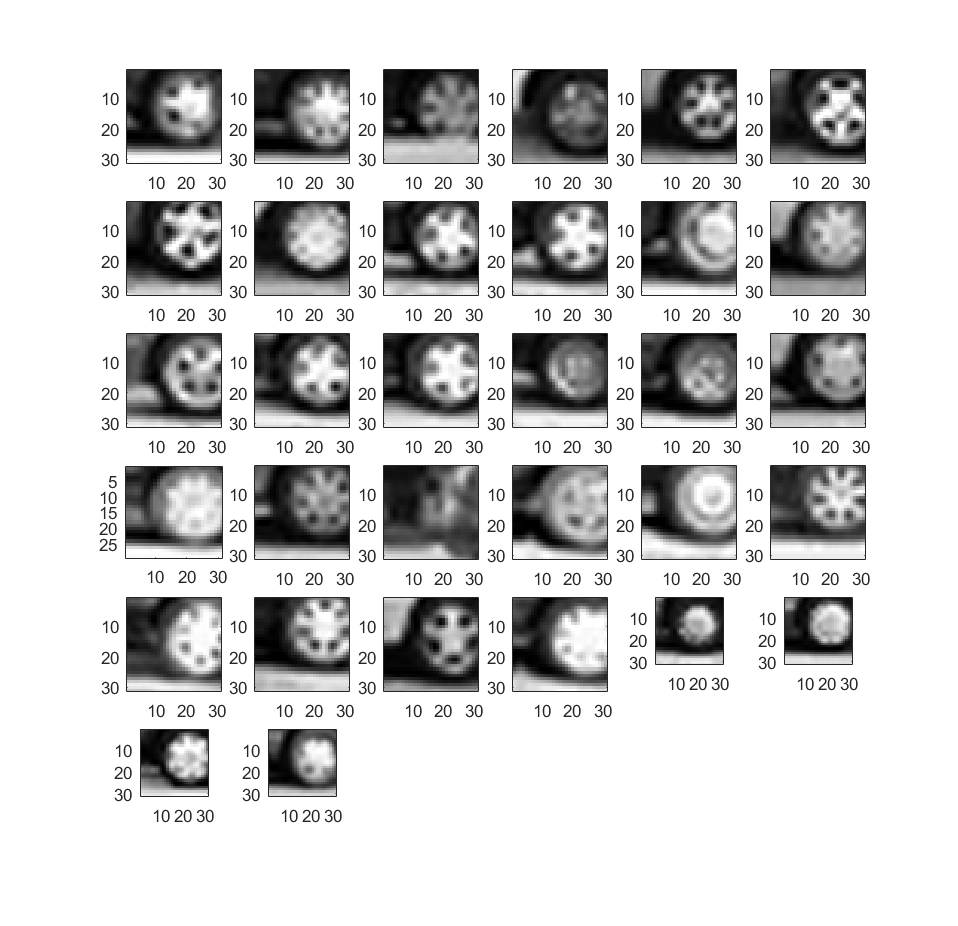
\includegraphics[width=0.5\textwidth]{features1}
	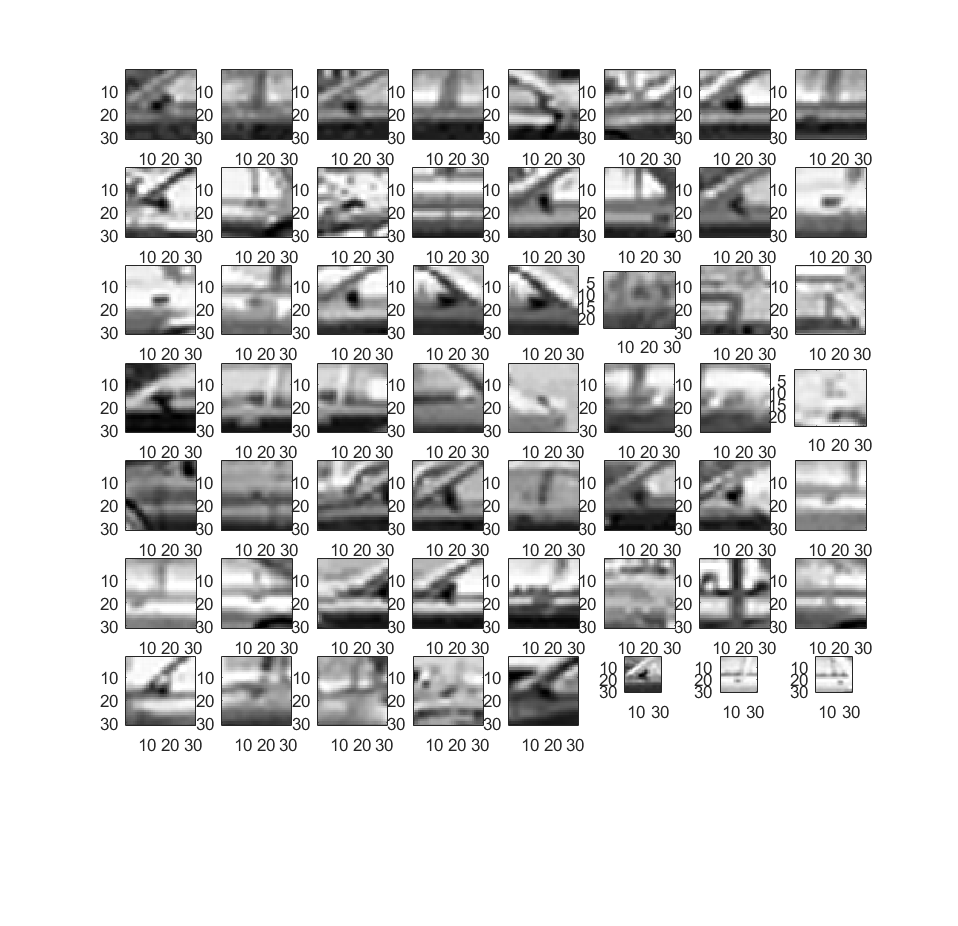
\includegraphics[width=0.5\textwidth]{features2}
	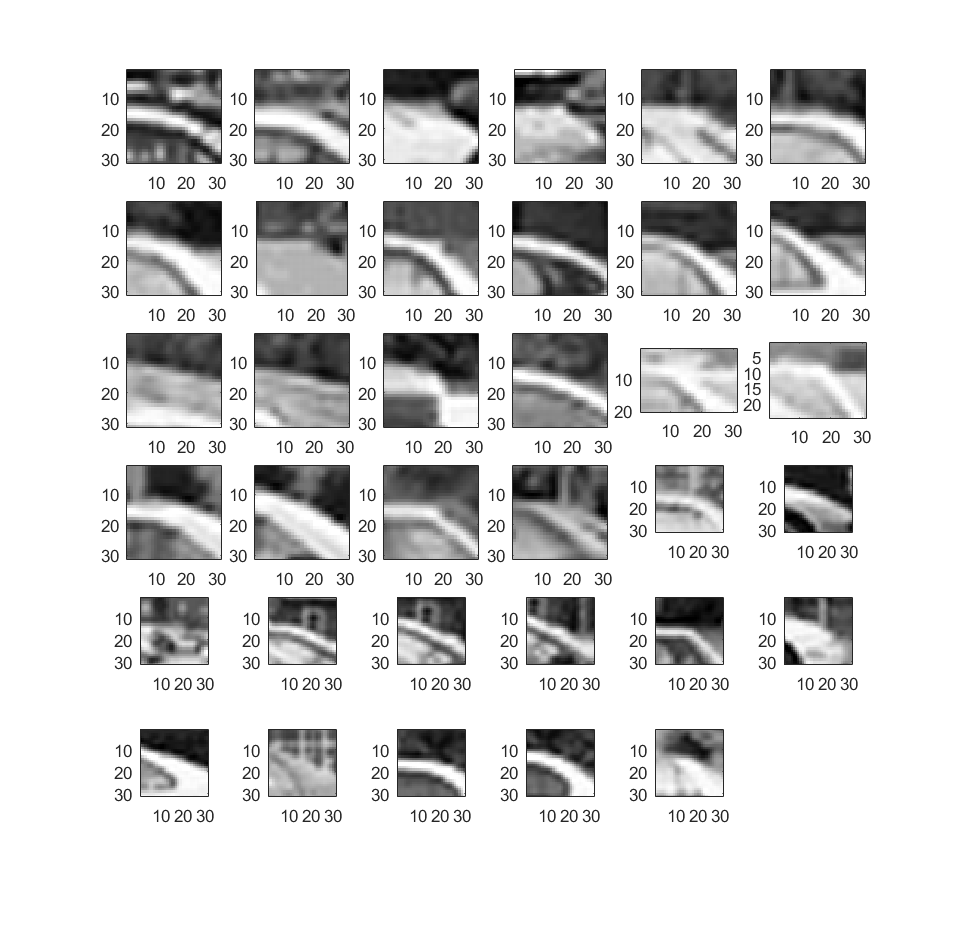
\includegraphics[width=0.5\textwidth]{features3}
	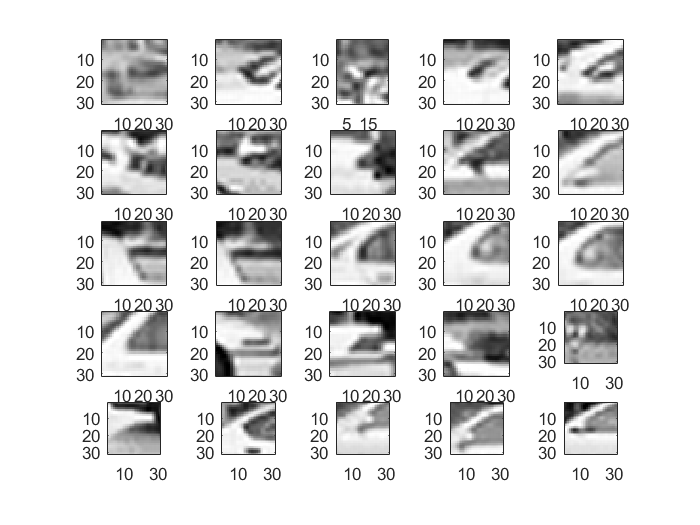
\includegraphics[width=0.5\textwidth]{features4}
		
	\caption{Visualization of several codebook entries. \textit{Upper left}: visualizes the wheels. \textit{Upper right}: the side mirror. \textit{Lower left} curvature in the back part of the roof. \textit{Lower right} appears to be the curvature, mainly in the passenger door window but it is not entirely clear.  }
\end{figure}
As we can see in Figure 1 the learned codebooks make sense from a visual point of view. They seem to capture shapes that are representative for a car. For instance on the upper left we can see the wheels of the car or on the upper right the side mirror. Other images are perhaps not so easily distinguishable, however they represent parts that one would mainly find in a car as opposed to, say, the environment such as the slope in the back part of the roof on the Lower left of Figure 1, or the edge of the passenger window.
\newpage
\section*{Question 2: Occurrence Generation}
\begin{figure}[H]
	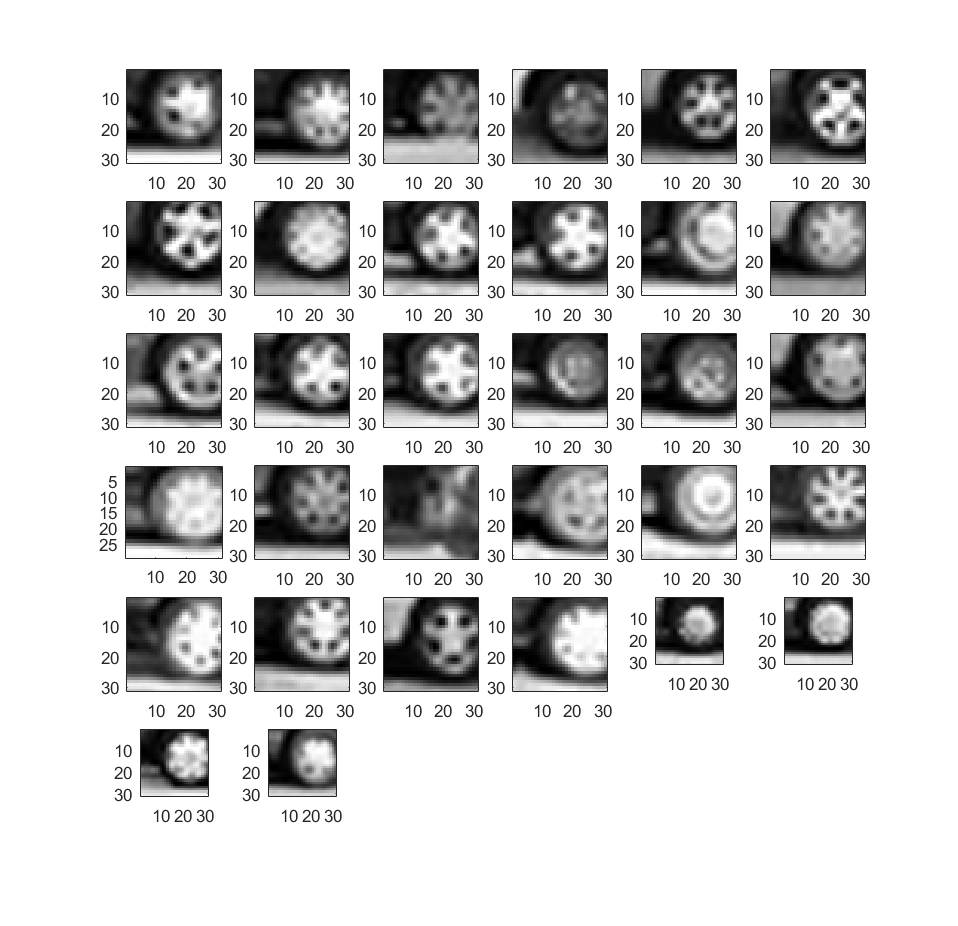
\includegraphics[width=0.5\textwidth]{features1}
	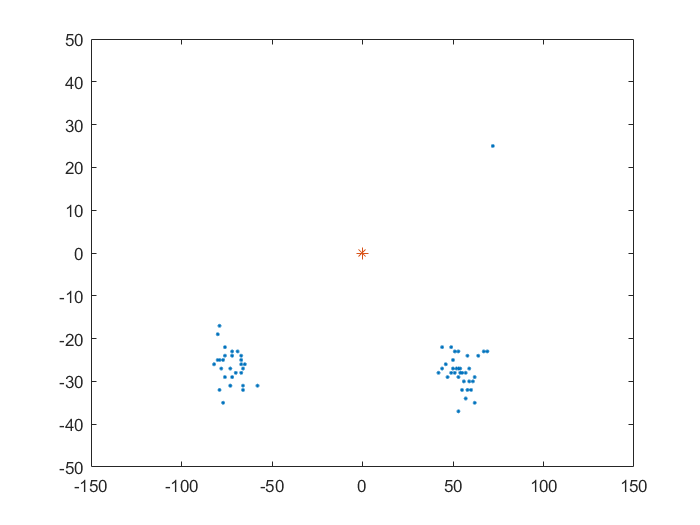
\includegraphics[width=0.5\textwidth]{clusters1}
	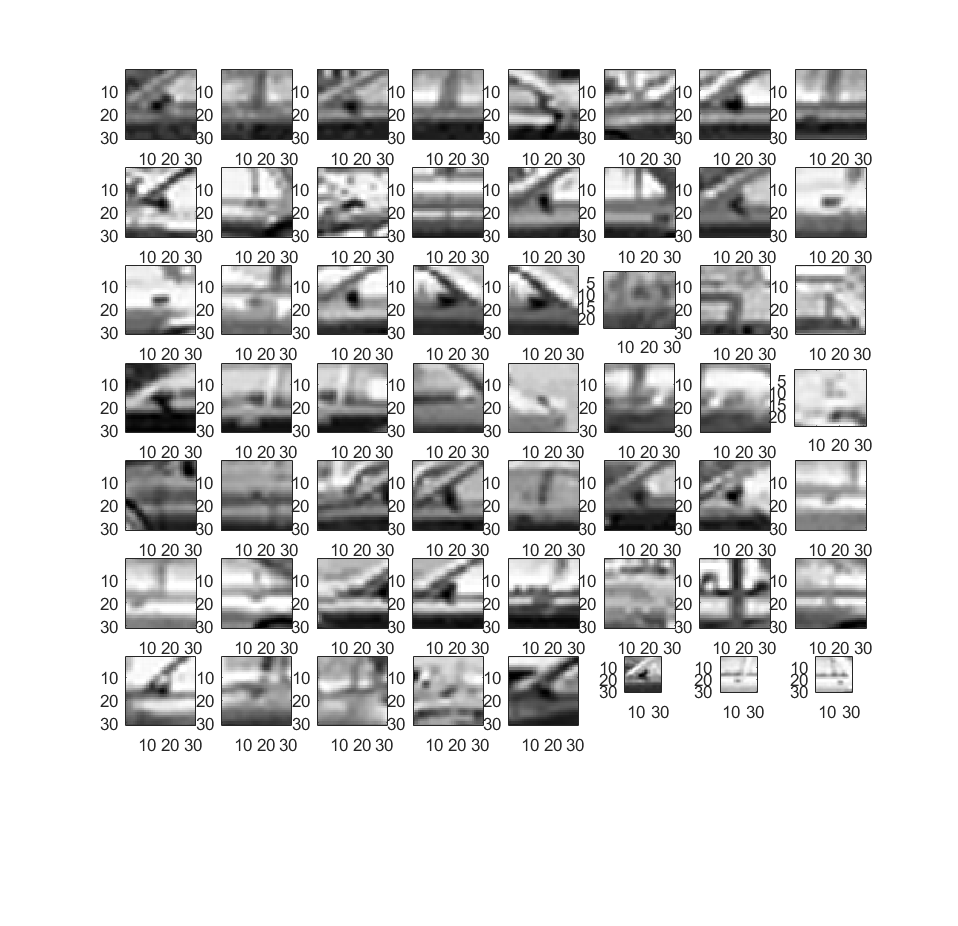
\includegraphics[width=0.5\textwidth]{features2}
	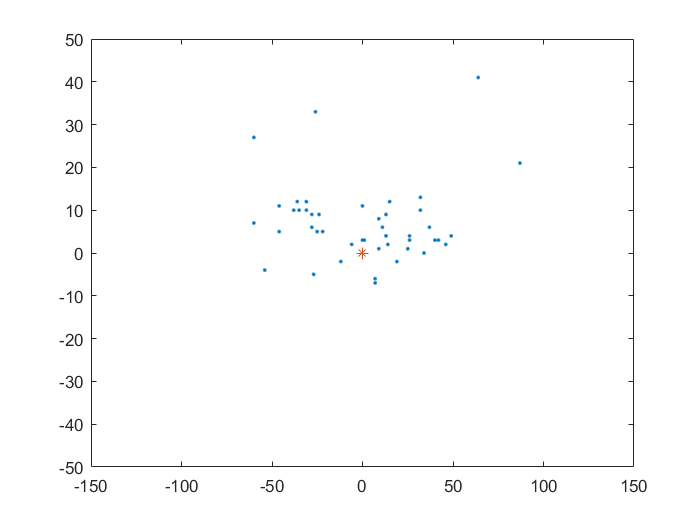
\includegraphics[width=0.5\textwidth]{clusters2}
	
	
	\caption{Visualization of occurrences together with their codebook entries discussed in Figure 1. \textit{Upper row}: visualizes the wheels. \textit{Lower row}: the side mirror. }
\end{figure}

From Figure 2 it is clear that the wheel occurrences are located where expected, we can see that by two small groups of points at approximately the same horizontal distance from the image center and in the lower part of the image, which matches our expectations of where to find the wheels of a car, unless there was an accident and the car is flipped around. There is one occurrence in the upper right part of the image, which is most likely, an outlier. 

As for the side mirror, it also matches one's expectations, about the middle in vertical position and what looks like two groups of occurrences close to the center in horizontal position representing cars facing both directions. There are a few more outliers (4) compared to the wheels, but it's still nothing to be surprised about.\\
\begin{figure}[H]
	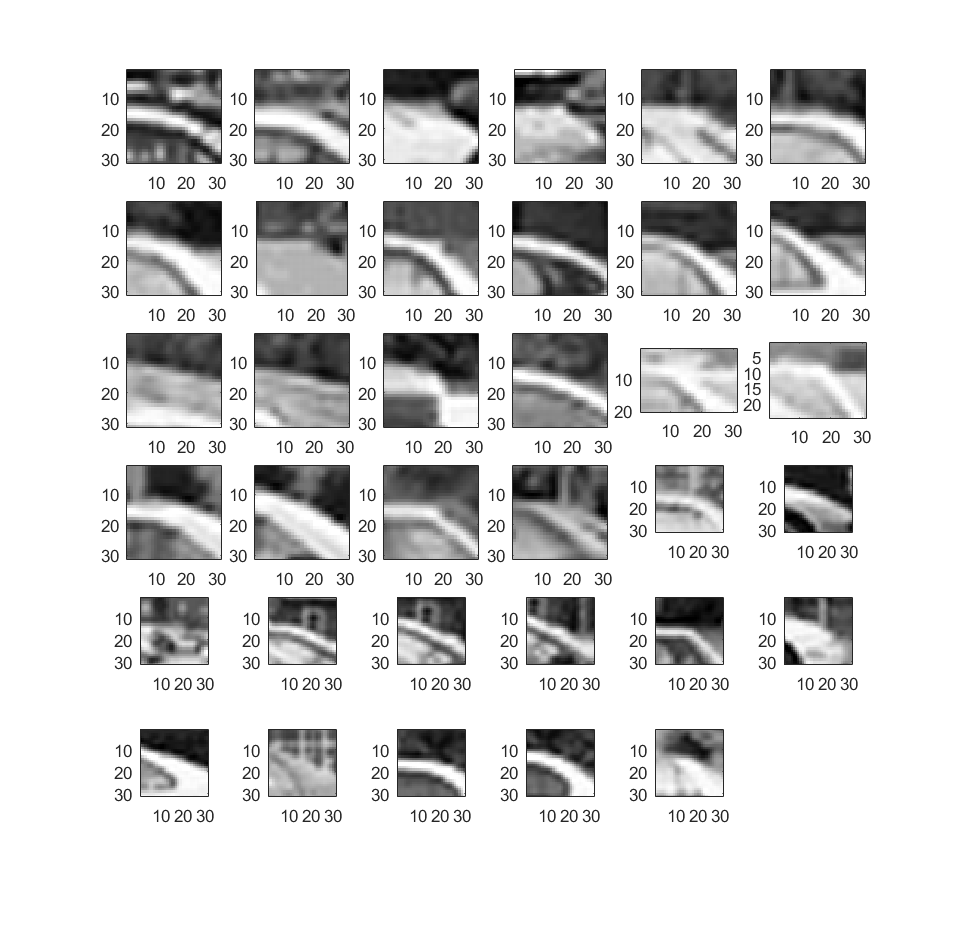
\includegraphics[width=0.5\textwidth]{features3}
	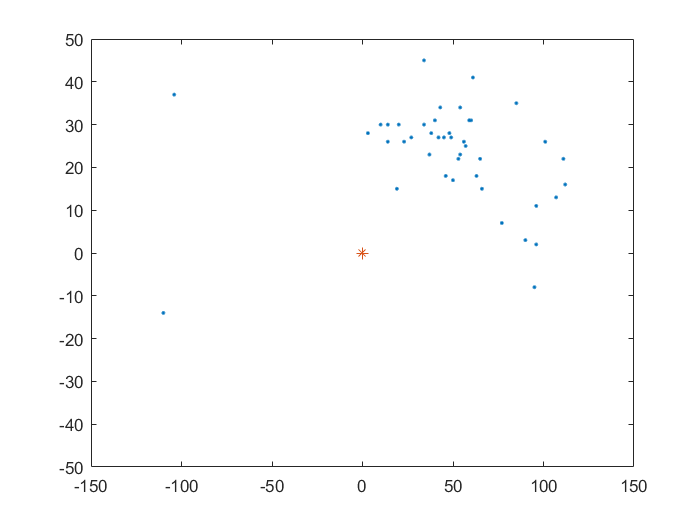
\includegraphics[width=0.5\textwidth]{clusters3}
	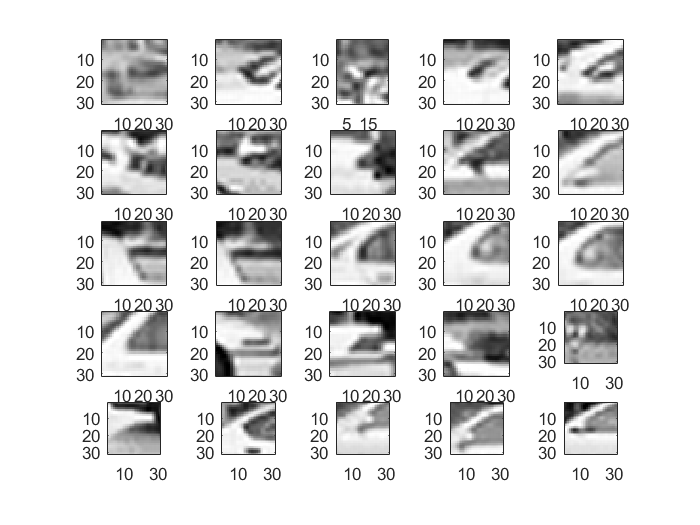
\includegraphics[width=0.5\textwidth]{features4}
	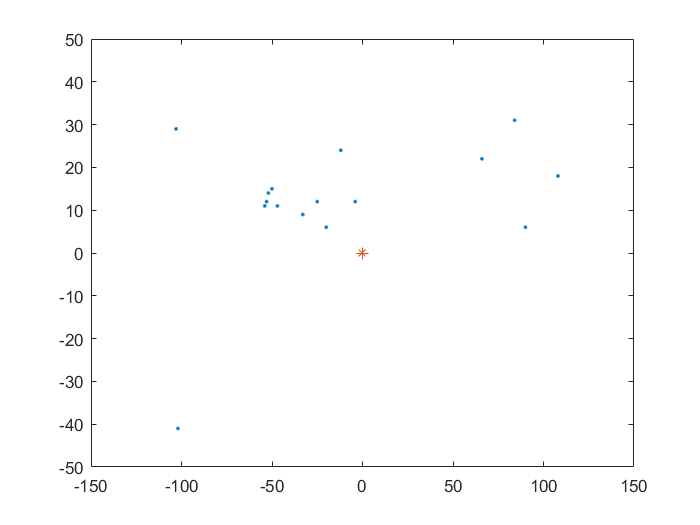
\includegraphics[width=0.5\textwidth]{clusters4}
	
	
	\caption{Visualization of occurrences together with their codebook entries. \textit{Upper row}: visualizes the roof. \textit{Lower row}: the passenger window. }
\end{figure}

	
	In the case of the car's roof the data is a little more spread. The core group is located approximately where one would expect it (towards the right and a little up) which matches the codebook images. The reason why, we're not seeing a mirrored group on the  right, as with the examples on Figure 2, is probably because the slope of the car is the opposite as if the car would be facing the right side of the image. Thus there probably exists another cluster that contains this mirrored group.
	
	Finally on the lower row of Figure 3, one can see a much smaller number of occurrences than in the previous clusters. The Codebook appears to focus mainly on the passenger window, but there are several exceptions including front windows, back and front parts of the car. The Codebook then probably captures some sharp edge which is more loosely defined than the aforementioned Codebooks and while being a little common in passenger seat windows, the car is not necessarily designed in that way, nor is this edge exclusive to the passenger seat window. It is then to be expected that the cluster is not as cohesive as the other ones.


\newpage
\section*{Question 3: Recognition}
For this exercise we draw the 3 most likely detections with highest score with a constant sized bounding box. 



\begin{figure}[H]
	\begin{center}
	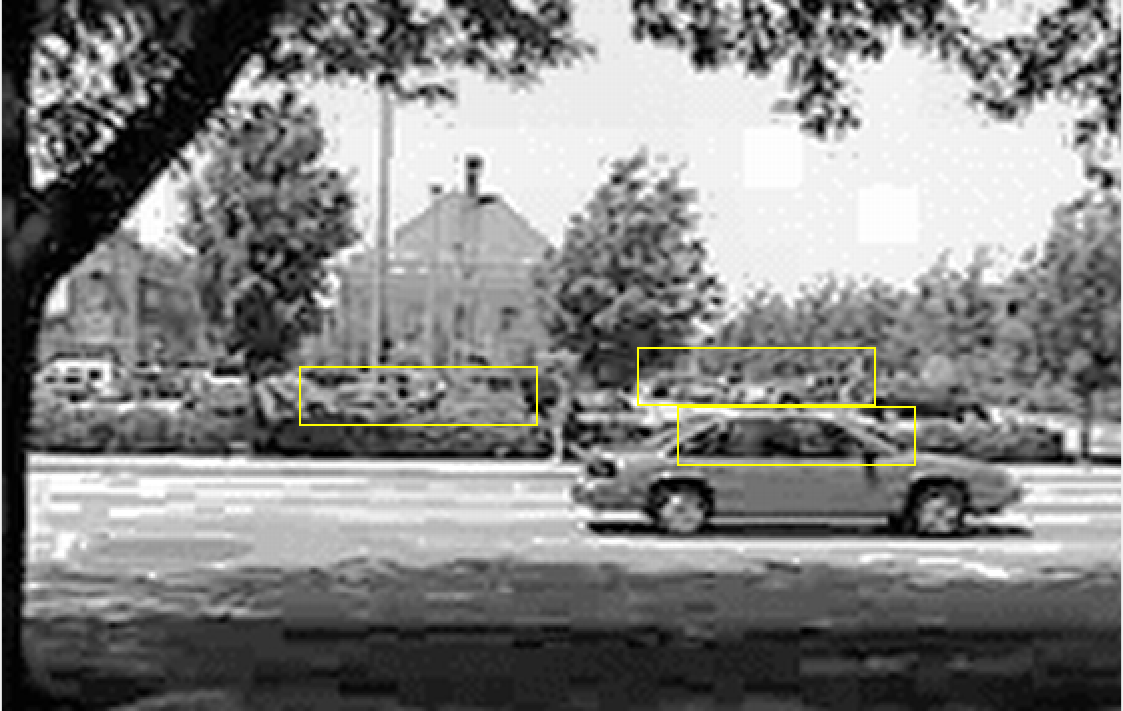
\includegraphics[width=0.5\textwidth]{eva2}
	
	\caption{Example of a correctly detected car }
\end{center}
\end{figure}
In this first example we see a car that is detected by one of the three most likely detections. A second detection is just above the previous one but also relatively close to the car. The third one is completely far off, but it is actually detecting some bushes as if it were a car.

\begin{figure}[H]
	\begin{center}
	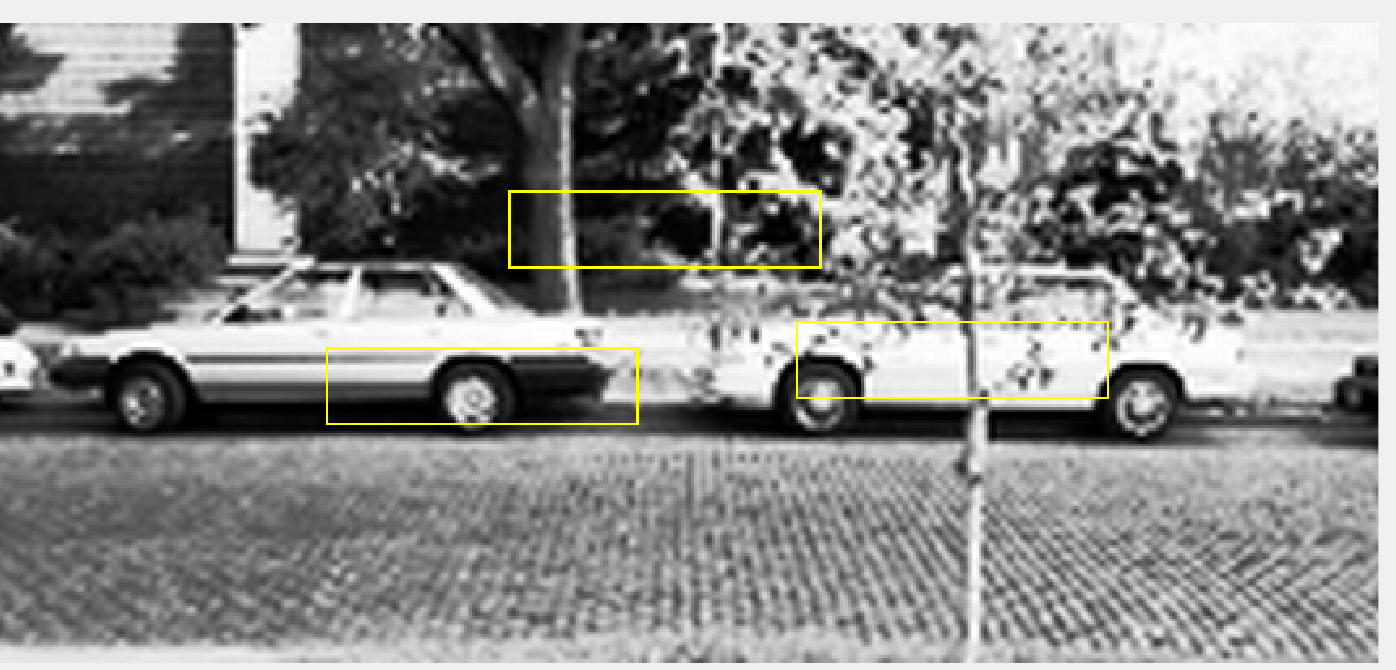
\includegraphics[width=0.5\textwidth]{eva1}
	\caption{Example of two correctly detected cars }
\end{center}
\end{figure}

In Figure2 one can see two cars, both of them are correctly detected by two of the three highest scoring detections. A third detection is found in between the cars. This might be a third hypothesis which gets confused because of the back wheels on the left car and the front wheels of the right car.


\begin{figure}[H]
	\begin{center}
	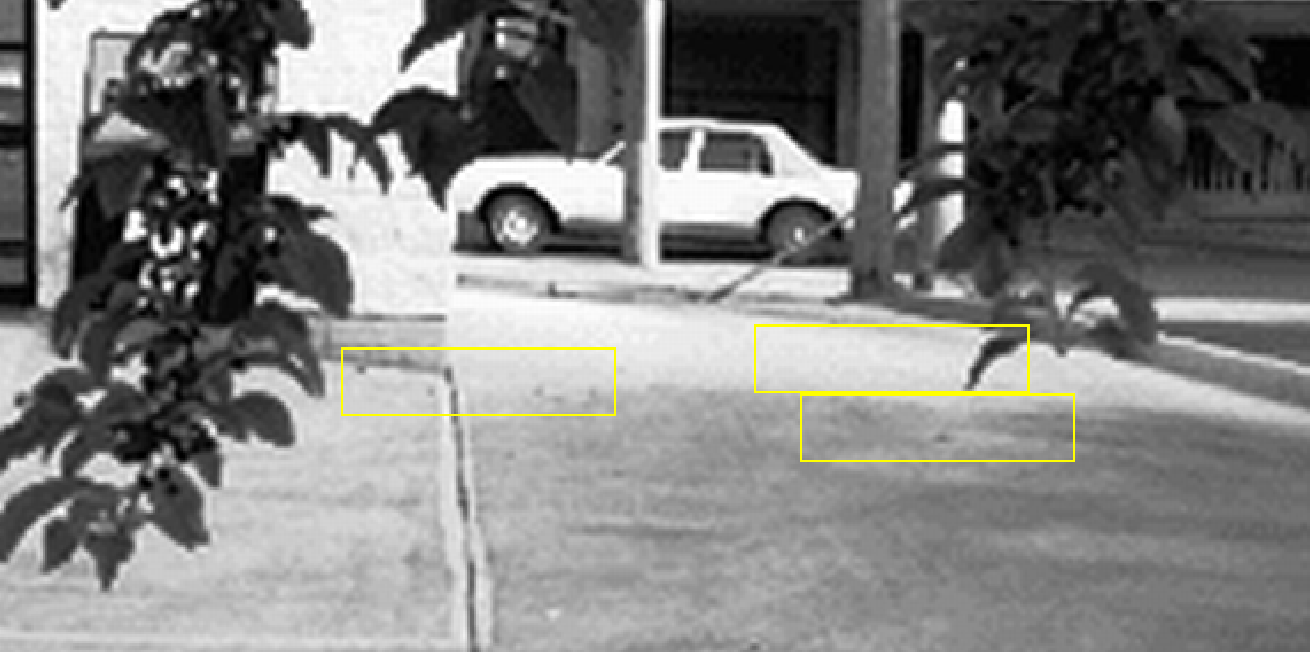
\includegraphics[width=0.5\textwidth]{eva3}
	\caption{Example of an incorrectly detected car }
\end{center}
\end{figure}

In Figure 3 we see a car that is partly occluded. All three of the highest detections are far off. Even though the car is in part hidden, one would expect that with the amount of visibility which still remains, an accurate detection should be possible, which leads us to think there is still an error in the code.

Regarding the first two examples, one can see from the Figure 2 for instance, that one possible improvement could be, as seen in the lecture, to reject based on bounding box overlap, this may however be a little problematic so instead using segmentations to resolve this ambiguities might be better.


\end{document}
